\documentclass{report}
\usepackage[a4paper, total={6in, 8in}]{geometry}
\usepackage{amsmath}
\usepackage{bm}
\usepackage{pgfplots}
\usepackage{ amssymb }
\usepackage{color, soul}
\usepackage[backend=biber]{biblatex}
\addbibresource{references.bib}
\graphicspath{{images/}}


%opening
\title{Literature Survey - (Title pending)}
\author{Ash}

\newcommand{\TODO}[1]{\sethlcolor{pink}\hl{\\(#1)\\}}
\newcommand{\FEEDBACK}[1]{\sethlcolor{green}\hl{\\ Feedback: \\#1\\}}
\newcommand{\TOCITE}[1]{\textsuperscript{\underline{citation needed #1}}}

\begin{document}
	
	\maketitle
	\thispagestyle{empty}
	\newpage
	\thispagestyle{empty}
	\tableofcontents
	\newpage
	\thispagestyle{empty}
	\listoffigures
	\newpage
	
	\chapter{Introduction}
	\TODO{Week 11}
	\textbf{Very brief background}
	Deep learning good for large data set.
	Motivation is to work with less training examples \\
	\textbf{Existing work on meta learning and continuous learning} \\
	\textbf{Gap the literature} \\
	\textbf{Describe the Problem}
	A system that can do continual learning. Refer to this doc:
	https://paper.dropbox.com/doc/Adding-classes-an-existing-classifier-RdKxXHh7M9OWbHvEvCCsV
	We want it to be scalable with respect to the number of classes
	So it should work faster than nearest neighbour based approaches for large number of classes \\
	\textbf{High level how you will solve it and why it is different from existing work} \\
	\textbf{Brief description of experimental setup} \\
	
	
	\chapter{Background}
	Images are sources of highly-dimensional data for which humans have the incredible ability of understanding. Developing computer vision systems that perform to even a similar capacity to that of humans is an inherently difficult task. The gift of easily converting pixel values into meaningful concepts is a skill that computer vision experts have been attempting to transfer to computers for decades. \par
	The ability to quickly gain an understanding of a new concept is a uniquely human trait. Consider that ter seeing a zebra only once, most humans would be able to easily identify it in a humorous police line-up  -- perhaps after the theft of a monkey's balloon --  but the best image recognition systems over the years would be dependant on seeing many examples of zebras. It is quite standard to present hundreds of examples of each new concept in order to learn which parts of the image data are unimportant noise, and which parts are characteristic. \par
	Modern techniques have made great advances in the application of meta-learning techniques (learning to learn) to few-shot learning; the task of having a computer vision system learn to recognize images from only a few labelled examples. While the results have been very encouraging, the problem of catastrophic forgetting persists. The challenge of continuous learning is to teach new classes to a system without interfering with the previously learnt tasks. \par
	Following on from the basic domain overview provided in chapter 1, we will now discuss neural-networks more thoroughly, and how advancements in the field have put us in a good position to tackle few-shot and continous learning. First we discuss the motivations for data-driven machine learning, the breadth of applicable tasks, and how these can be achieved. We will end with the problems regularly encountered with small data-sets and how modern architectures seek to resolve these. \par
	
	\section{Hand Engineered and Learnt Features} \label{hand-eng:1}
	Features are a general term for characteristic attributes which exist across all samples in a data-set or domain. These features were traditionally hansd-engineered by machine learning experts, carefully selecting the base-components of which the data-set in question appears to comprise. A common hand-engineered feature is the Histogram of Oriented Gradients (fig \ref{fig:hog:1}), which results in small regions of an image voting on the best description of the local gradient. \par
	However, a fundamental problem with hand-engineered features is that it imposes human knowledge onto a problem to be solved by a computer. Furthermore, key features for complex data such as images and video are incredibly difficult to ascertain -- especially if desiring generic, transferable features. With the rise of neural networks -- specifically CNNs, which will be discussed in detail later -- feature-learning has become the norm. This essentially takes the task of feature engineering and solves it in a data-driven manner. \par
	\begin{figure}[!h]
		\centering
		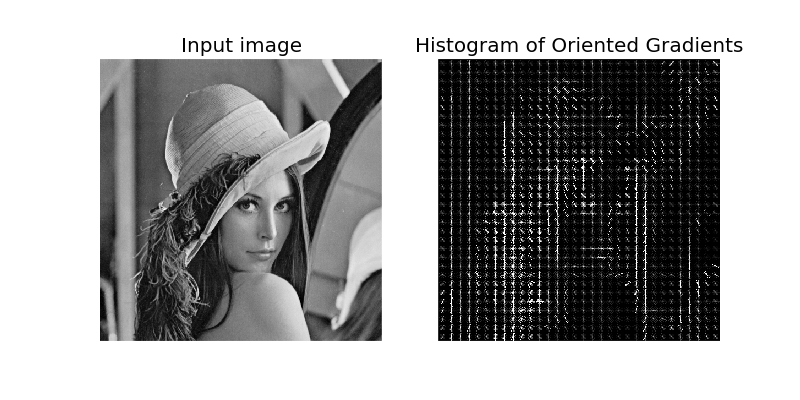
\includegraphics[width=11cm]{hog}
		\caption{Histogram of Oriented Gradients}
		\label{fig:hog:1}
	\end{figure}

	\section{Supervised Learning}
	Supervised learning is a machine learning strategy whereby the target solution is presented after each training iteration. This differs from unsupervised learning in that unsupervised learning has no direct target to learn from and is used to find underlying commonalities or patterns in data. \par
	Supervised learning is the most commonly used method for image and video tasks, as typically the objective is to perform tasks where the target is well-defined. Common supervised learning tasks are \emph{image classification} - where the objective is to assign an input image a label from a fixed set of categories; \emph{localisation} - where the objective is to produce the coordinates of an object of interest from the input image; and \emph{detection} - which combines the previous two tasks. The task of localisation is actually a specific use-case for \emph{regression}, where the system is to predict a real-valued scalar given some input - used frequently for finance and weather prediction among others. \par
	There are a multitude of supervised and unsupervised learning problems, with  almost all meta-learning strategies targeting supervised learning. Due to this -- and that supervised learning has clearer, more measurable results -- I will focus primarily on the supervised task of image classification using neural networks. \par
	

	\section{Optimisation}
	\subsection{Loss} \label{loss:1}
	The process of optimising a machine learning system is to present it with a target of some sort -- either in the supervised or unsupervised setting -- and compute a numerical quantity called \textit{loss} or \textit{cost}. The loss is a scalar value which is representative of how ``badly'' the system has performed inference given the input image. It is the system's objective to minimise this value through some optimisation algorithm. The loss function is specifically chosen for the task at hand, \textit{cross-entropy} being a common choice for image classification tasks and \textit{mean-squared (L2) error}  for regression. \\
	
	\subsubsection{Symbols}
	Before discussing loss functions, it's important to understand the inputs and outputs of a machine learning system when performing image classification. \par
	For a system that makes predictions between $N$ classes, its input is a vector of image features $\bm{x}$ - usually the raw pixel values. The system's output is a vector $\bm{\hat{y}}$ of length $N$, where each of the output values $\bm{\hat{y}}_i$ is a score for class $i$ being the correct answer. The loss $\mathcal{L}$, as described above, is a function of the predictions $\bm{\hat{y}}$ and the target values $\bm{y}$. The target values are typically encoded as a \textit{one-hot} vector of length $N$, which is all zeros with a 1 in the position of the correct class. \\
	
	\subsubsection{Softmax}
	As the system's outputs aren't normalised and thus cannot be interpreted as a true confidence measure, the outputs normally go through a softmax function $\sigma$.
	\begin{equation} \label{softmax:1}
	 \sigma(\bm{\hat{y}})_i = \frac{e^{\hat{y}_i}}{\sum_{k=1}^{N}e^{\hat{y}_i}} \\
	\end{equation}                                                              
	The softmax function (eq \ref{softmax:1}) squashes the arbitrary scores into a vector such that its values sum to $1$ and are each in the range $[0, 1]$. The resultant values can be interpreted as the probability of the input image falling into each of the classes. Figure \ref{fig:softmax:1} shows the raw, unscaled predictions from a classification network (red), and the results of applying the softmax function (green). \par
	\begin{figure}[h] 
		\centering
		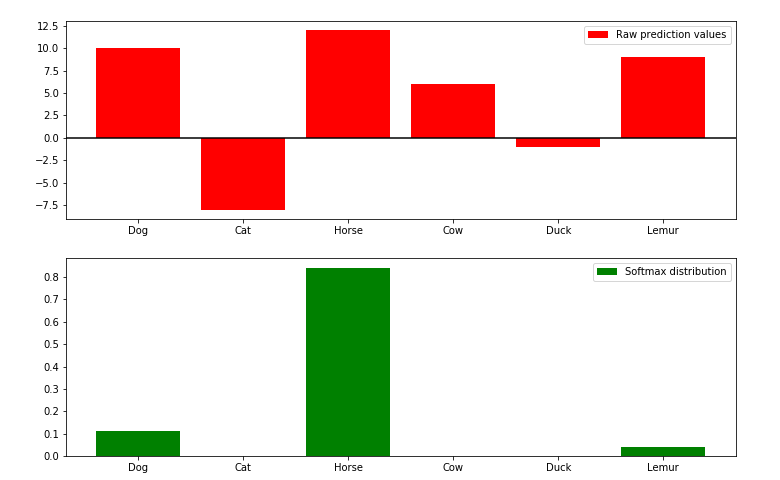
\includegraphics[width=12cm]{softmaxplot}
		\caption{The Softmax function applied to classification outputs}
		Note how the softmax function preserves the ordering of prediction values while emphasizing their differences, and gives the required properties of a probability distribution.
		\label{fig:softmax:1}
	\end{figure}
	
	\subsubsection{Cross-Entropy Loss}	
	With the machine learning system producing a normalised probability distribution across classes, those values need be compared with the targets to produce a scalar loss value. 
	Cross-entropy loss, otherwise known as \textit{log loss}, penalises for differences between predicted values and targets, with the penalty growing harsher for further-away predictions as demonstrated in fig \ref{fig:cross-entropy:1}.\\
	For a vector of predictions $\bm{\hat{y}}$ and a one-hot target vector $\bm{y}$, the cross-entropy loss is:r
	\begin{equation} \label{cross-entropy:1}
	 H(\bm{\hat{y}}, \bm{y}) = - \sum_{k=1}^{N}y_k log(\hat{y}_k) \\
	\end{equation}  
	For the special case of \textit{binary} cross-entropy (as shown in fig \ref{fig:cross-entropy:1}) where number of classes $N$ is 2, the network's outputs are generally reduced to a single scalar value and cross entropy calculated as:
	\begin{equation} \label{cross-entropy:2}
	 H(\hat{y}, y) = -(y log(\hat{y}) + (1 - y)log(1-\hat{y})
	\end{equation}
	\begin{figure}[!h]
		\centering
			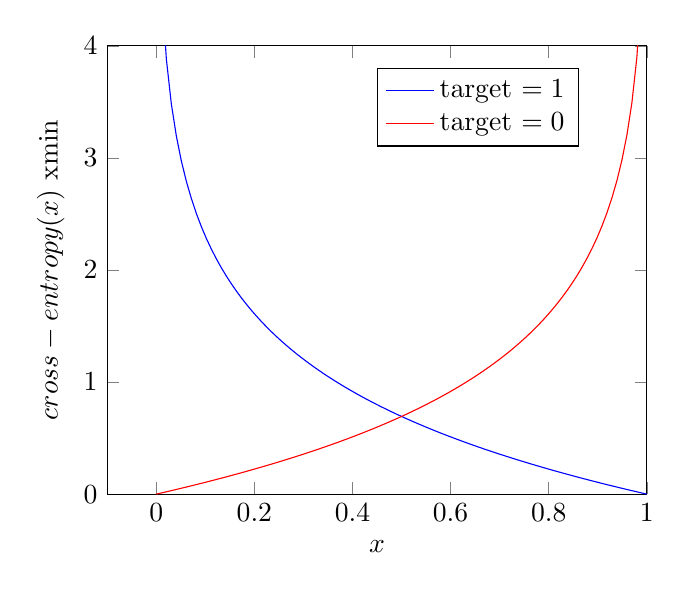
\begin{tikzpicture}
			\begin{axis}[ 
			xlabel=$x$,
			ylabel={$cross-entropy(x)$}
			xmin=0, xmax=1,
			ymin=0, ymax=4,
			legend style={at={(0.5,0.95)},anchor=north west}
			] 
			\addplot[domain=-0.01:1, color=blue, samples=100] 
				{-ln(x)};
			\addplot[domain=0:1, color=red, samples=100]
				{-ln(1 - x)};
			\addlegendentry{target $=1$}
			\addlegendentry{target $=0$}
			\end{axis}
			\end{tikzpicture}
			\caption{Binary Cross-Entropy}
			\label{fig:cross-entropy:1}
	\end{figure}
	
	\subsubsection{Mean-Squared Error (L2)}
	Mean-squared error is used for regression tasks, where the objective is to predict a quantitative value rather than a measure of probability. As L2 loss minimises the average error between the predictions $\bm{\hat{y}}$ and targets $\bm{y}$, the system learns to make predictions which lie in the mean position of these, which is generally ideal for regression tasks where there is one solution.\\
	\begin{equation} \label{mean-squared-error:1}
	 L2(\hat{\bm{y}}, \bm{y}) = \sum_{k=1}^{N}(y_k - \hat{y}_k)^2
	\end{equation}
	
	\section{Neural Networks}
	Artifical Neural Networks (\textit{ANNs}) are machine learning systems loosely inspired by the functioning of the biological neural networks of the brain. They are composed of artificial neurons which transmit signals from one another in the form of a non-linear function of the sum of the incoming inputs. ANNs model unknown functions of arbitrary complexity, with their representational power a function of their size. \par
	If we look at the structure of the simplest neuron possible $f_1$ (figure \ref{fig:neurons:1}a) we see that it is composed of two components - a weight $w_1$ and a bias $b_1$. Passing a value $x$ through a neuron $f_1$ is equivalent to computing the linear function $f_1(x) = w_1x + b_1$. The output of a neuron is known as its ``activation'' -- how activated the neuron was given that input.
	If the outputs of this neuron are then passed into a similar neuron $f_2$, we end up with the composite function 
	\begin{align}
	 (f_2\circ f_1)(x) &= (w_2(w_1x + b_1) + b_2) \\
	 &= w_2w_1x + b_1w_2 + b_2	
	\end{align}
	which is still a linear function of $x$. This is true for any number of sequential neurons, meaning that any composition of linear neurons is only as good as a single neuron. Having the capacity to produce linear relationships is only useful if the function being modelled is, itself, a linear function. For more complex modelling tasks -- which are encountered more often than not -- non-linearities need to be introduced into the network. In making a neuron a non-linear function, the problem with composite functions noted above no-longer exists; adding additional neurons increases the representational power of the model. \par
	
	\subsection{Activation Functions / Non-Linearities}
	Activation functions (also known as non-linearities) are a critical component of neural networks as they add the capacity to model non-linear relationships. The inspiration for activation functions is drawn -- once again -- from the operation of biological neural networks, whereby neurons are only ``activated'' given sufficient input signal. In modern neural networks there are only a few activation functions regularly used: \par


	\begin{itemize}
		\item\textbf{Sigmoid} $= \frac{1}{1 + e^{-x}}$ : The Sigmoid activation function (also known as the \textit{logistic function}) has the nice property that $(\forall x \in \mathbb{R}) Sigmoid(x)\in(0, 1)$ which is useful as a way of normalising values, especially when the output is to be interpreted as a probability.
		
		\item\textbf{TanH} $= \frac{e^{2x} - 1}{e^{2x} + 1}$ : The hyperbolic tangent function is similar to sigmoid, but maps numbers to the range $(-1, 1)$.
		
		\item\textbf{ReLU} $= \begin{cases}
		0, & \text{if } x < 0 \\
		x, & \text{if } x \ge 0 \\
		\end{cases}$
		The Rectified Linear Unit maps numbers to the range $[0, \infty)$ and has the advantage that it is much more computationally efficient than the above two activation functions; in most cases it yields better results.
		\item\textbf{Leaky ReLU} $= \begin{cases}
		0.01x, & \text{if } x < 0 \\
		x, & \text{if } x \ge 0 \\
		\end{cases}$
		The Leaky Rectified Linear Unit operates like ReLU, but allows numbers less than zero to ``leak'' through - this is helpful during \textit{backpropogation}, which is discussed at length in section \ref{backprop:1}.
	\end{itemize}

	\subsection{Fully-Connected Layers} \label{fully-connected:1}
	The arrangement and structure of neurons discussed thus far hasn't been very practical, in that we were only considering a chain of continuous neurons one after another with only one input and output. Neurons will typically receive multiple inputs and produce a weighted sum of those inputs (fig \ref{fig:neurons:1}b). A neuron given $N$ inputs $x_i$ with weights $w_i$ and bias $b$ would then form the linear equation $w_1x_1 + w_2x_2 + ... + w_Nx_N + b$. \textit{For our purposes we will consider the activation function to be inside each neuron, although in practice they are applied in a layered manner.} \par
	For a system consisting of multiple inputs, we want to allow diverse interactions between them. This is achieved by what's known as a \textit{Fully-Connected Layer} of neurons, where each output from the previous layer is passed as input to each of the following layer's neurons. Networks are generally grouped into layers to provide a nice abstraction away from the hundreds or thousands of neurons inside. The layer architecture of neural networks means that each layer can be considered a stand-alone block, a black box with a mapping from an an arbitrary input size to an arbitrary output size. They can therefore be stacked on top of each-other to form a \textit{fully-connected neural network} - see figure \ref{fig:neurons:1}c for an example. \par
	A valid interpretation of the weights in a neural network is to consider them a measure of the importance of the inputs for the corresponding output. For example, a network which predicts the price of a house given the number of bedrooms; square metres; and the window-thickness, will likely have a very small weight for the window-thickness as it's not very \textit{important} to the price prediction. This is a very literal example, and with more complex tasks such as image classification the weights are not as easily interpretable. \par
	\begin{figure}[h]
		\centering
		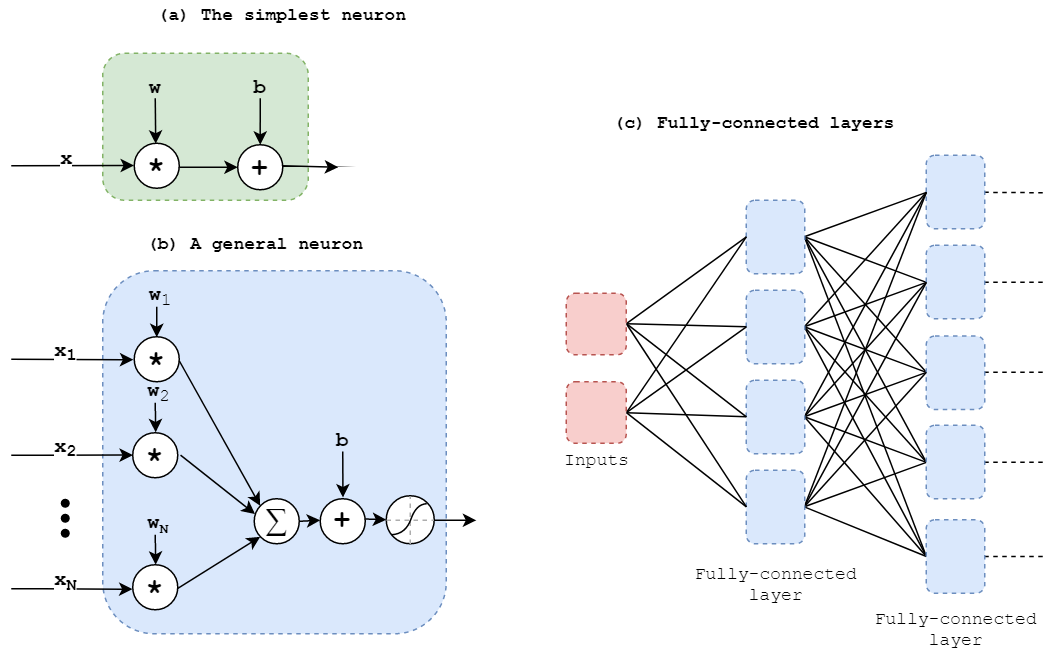
\includegraphics[width=14cm]{neurons}
		\caption{Neurons and fully-connected layers}
		\label{fig:neurons:1}
	\end{figure}

	\subsection{Stochastic Gradient Descent (SGD)} \label{sgd:1}
	An ANN begins with randomly generated weights and biases $\bm{W}$ and $\bm{B}$, which are collectively referred to as the ``parameters'' or ``weights'' and indicated by $\bm{\theta}$. The objective of an ANN is to select weights $\bm{\theta}$ that minimise the error computed by the loss function $\mathcal{L}$ (section \ref{loss:1}). Linear functions $f(\bm{x}, \bm{\theta})$ can be minimised by analytical techniques, but complex neural networks must be iteratively optimised by numerical methods. \par
	With the loss between a prediction $\hat{y}$ and target $y$, we can compute the gradients of the parameters and make a small step in the direction which will reduce the loss for the given example (see figure \ref{fig:grad-descent:1}). When performing this operation over the entire data-set at once, this is known as gradient descent. This is usually not an option as the computational resources required for full gradient descent are prohibitive. If we instead repeat this operation for different examples until we have stabilised the loss to a low value, we have Stochastic Gradient Descent. The most common variant to this technique is known as Batch Gradient Descent, where instead of computing the loss and performing an update to the parameters on a per-example basis, the process is applied once per \textit{batch} of examples. It facilitates more stable learning, as the loss doesn't fluctuate as much as between single examples. Batch Gradient Descent is the basis for most ANN optimisation, although we'll discuss modern variants in section \ref{optimizers:1}. \par
		\begin{figure}[h]
		\centering
		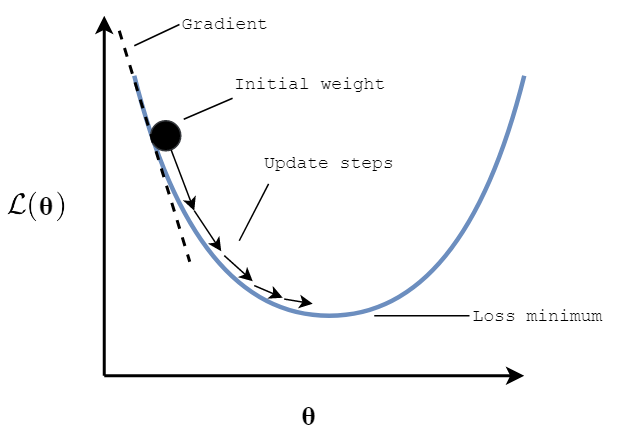
\includegraphics[width=9cm]{graddescent}
		\caption{Gradient descent updates}
		\label{fig:grad-descent:1}
	\end{figure}

	\subsection{Gradients and Backpropagation} \label{backprop:1}
	We shall consider a general ANN $\sigma$ with $2$ fully-connected layers $f_1, f_2$ parameterised by $\bm{\theta} = \{\bm{\theta}_1, \bm{\theta}_2\}$ which can be represented as:
	\begin{align} \label{gradients:1}
	 \bm{\hat{y}} = \sigma(\bm{x}, \bm{\theta}) = f_2(f_1(\bm{x},  \bm{\theta}_1), \bm{\theta}_2)
	\end{align}
	That is, the input $\bm{x}$ is fed through layer $f_1$ then $f_2$. We will also consider an arbitrary loss function $\mathcal{L}$ which compares the predictions $\bm{\hat{y}}$ with targets $\bm{y}$ and produces a scalar loss value:
	\begin{align}
	 \mathcal{L}(\bm{\hat{y}}, \bm{y})
	\end{align}
	As the input $\bm{x}$ and target $\bm{y}$ is fixed, we may only change the parameters $\bm{\theta}$ to improve the loss. As explained in section \ref{sgd:1}, we wish to make incremental changes to our parameters where each change decreases our loss value. We do so by computing the gradient of the parameters with respect to the loss value:
	\begin{align}
	 \frac{\partial\mathcal{L}(\bm{\hat{y}},\bm{y})}
	 {\partial\bm{\theta}}
	\end{align}
	If we are to find the gradients of the loss function with respect to the final layer's weights, we will have the equation
	\begin{align}
	\frac{\partial\mathcal{L}(\bm{\hat{y}},\bm{y})}
	{\partial\bm{\theta}_2}
	\end{align}
	which is considered to be easily calculable. However, if we wish to find the gradient of weights further towards the start of the network, we cannot work those out directly and instead need to make use of the differentiation chain rule: \par
	\begin{align}
	\frac{\partial f}{\partial x} = \frac{\partial f}{\partial u} \frac{\partial u}{\partial x}
	\end{align}
	To find the gradient of the loss function with respect to the first layer's weights, and considering that $\frac{\partial\mathcal{L}(\bm{\hat{y}},\bm{y})}
	{\partial\bm{\theta}_2}$ is calculable, we simply need apply the chain rule as such:
	\begin{align}
	\frac{\partial\mathcal{L}(\bm{\hat{y}},\bm{y})}{\partial\bm{\theta}_1} =
	\frac{\partial\mathcal{L}(\bm{\hat{y}},\bm{y})}
	{\partial\bm{\theta}_2}
	\frac{\partial\bm{\theta}_2}
	{\partial\bm{\theta}_1} 
	\end{align}
	That is, once we know the gradient of the loss with respect to the second layer's weights, we can compute the gradient of the second layer's weights with respect to the first layer's weights and multiply the two to find the gradient of the loss with respect to the first layer's weights. This generalises to neural networks with any number of layers of differing types. This is an intuitive relationship, as we are essentially calculating the compound contribution that a change in any one parameter's value will have on the final output -- the loss.  \par
	This technique used since the 1970s \parencite{backprop} is aptly named \textit{backpropagation of error gradient}, as it involves the propagation of the gradient of the error -- or loss -- from the end of the network back. \par
	Returning to the concept of SGD (section \ref{sgd:1}) which was introduced on a conceptual level, we can now delve deeper into the application of the algorithm. Assuming that we have computed the gradient of each parameter in the network for the given examples in our batch, we can visualise this as a ``loss landscape'', whereby moving the parameters down-hill results in a reduction in the loss. Adjusting a parameter by the negative of the gradient will result in a ``step'' that moves the parameter closer to a local minimum, with the objective to reach the lowest point possible. A configurable hyperparameter is the \textit{learning-rate}, commonly represented by $\alpha$, which is the ``size'' of the step to take - that is, the coefficient of the negative of the gradient to apply (eqn. \ref{sgd:1}). \par
	\begin{align} \label{sgd:1}
		\bm{\theta} = \bm{\theta} - \alpha \Delta_{\bm{\theta}} \mathcal{L}(\bm{\theta}, \bm{\hat{y}}, \bm{y})
	\end{align}
	\textit{For brevity we will from now write the gradient of the parameters $\bm{\theta}$ with respect to the loss function $\mathcal{L}$ as $\Delta_{\bm{\theta}} \mathcal{L}(\bm{\theta})$.} \\
	The problem that is quickly encountered is how large a value to set the learning rate $\alpha$. Too small a step and it will take a long time to reach a minimum; too large and you may over-shoot it (see figure \ref{fig:learning-rate:1}). The example in figure \ref{fig:learning-rate:1} is a very low-dimensional loss landscape where the correct direction to move seems very logical, but higher dimensional spaces with a greater number of parameters result in complex landscapes with many local minima. We also want to slow down when nearing the bottom of a minimum so we can properly reach the lowest point. If we take this into consideration, and the fact that for any mini-batch the loss landscape will be different due to noise in small sample sizes, choosing a fixed learning rate becomes problematic. In practice, many people simply set up a learning rate schedule, where they decrease the learning rate at intervals, but it is hard to get right. It is with this in mind that adaptive optimizers came about. \par
	\begin{figure}[h]
		\centering
		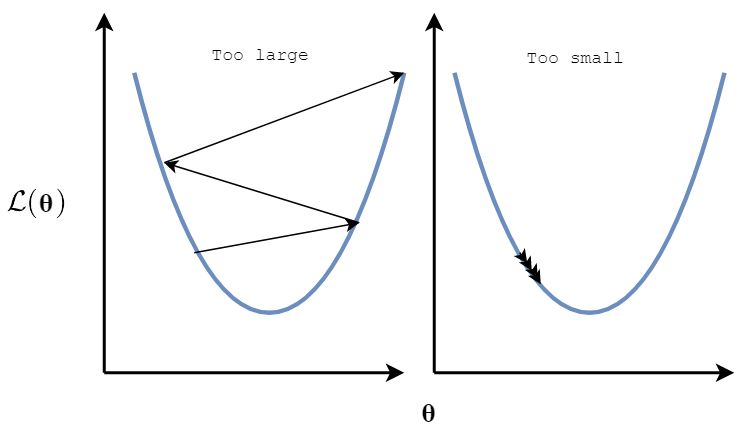
\includegraphics[width=10cm]{learningrate}
		\caption{Learning rate values}
		\label{fig:learning-rate:1}
	\end{figure}
	
	\subsection{Adaptive Optimizers} \label{optimizers:1}
	If we consider a data-set whereby each mini-batch has some noise but that there is an optimal parameterisation for the entire set, we could visualise the loss landscape as shifting slightly for each mini-batch, but where there is a common direction towards which most samples will lead. Standard SGD will just apply a fixed step-size for all updates which leads the parameters to oscillate along the greatest descent angle, regardless of past updates. \par
	
	\subsubsection{SGD with Momentum}
	It is with the idea of a consistent optimization direction that momentum \parencite{backprop} comes into play. This is a technique of updating parameters while taking past updates into consideration to find the ``common direction'' in which to move. This is done by using an update vector which intuitively acts like the momentum of a ball rolling down a hill. For any update step, the direction vector is updated with a scaled contribution from the current gradient direction, and that vector is used to update the parameters. It essentially dampens oscillating movement, as the direction vector compounds contributions in the same direction as given in the following equation
	\begin{align}
		\bm{v}_t &= \gamma \bm{v}_{t-1} + \alpha \Delta_{\bm{\theta}} \mathcal{L}(\bm{\theta}) \\
		\bm{\theta}_t &= \bm{\theta}_{t-1} - \bm{v}_t
	\end{align}
	where $\gamma$ is the momentum term which indicates how much movement we wish to carry forward from previous time-steps.
	
	\subsubsection{Nesterov Accelerated Gradient Descent}
	If we consider momentum to compound the previous slopes such as a ball rolling down a hill, we end up with a problem where the momentum may cause the parameters to overshoot the minimum. Nesterov Accelerated Gradient Descent \parencite{nesterov} pre-emptively considers post-step parameters and makes adjustments to the step \textit{actually} taken. It does so by approximating the position after a momentum parameter update ($\bm{\theta} - \gamma\bm{v}_{t-1}$), and computes the loss gradient not with respect to the current parameters, but to the approximate future position of the parameters. This optimisation strategy essentially glances into the future and makes a pre-emptive correction.
	\begin{align}
		\bm{v}_t &= \gamma \bm{v}_{t-1} + \alpha \Delta_{\bm{\theta}} \mathcal{L}(\bm{\theta} - \gamma\bm{v}_{t-1}) \\
		\bm{\theta}_t &= \bm{\theta}_{t-1} - \bm{v}_t
	\end{align}
	
	\subsubsection{Adagrad}
	Adagrad \parencite{adagrad} is the first of the true ``adaptive'' optimizers, in that it adjusts the learning rate on a per-parameter basis, taking past gradients into consideration. The Adagrad update rule is
	\begin{align} \label{adagrad:1}
		\theta_{t, i} &= \theta_{t-1, i} - \frac{\gamma}{\sqrt{g_{t, i} + \epsilon}} \mathcal{L}(\theta_{t, i})
	\end{align}
	where $\theta_i$ is the $i$th parameter, $\gamma$ is the learning rate, $g_i$ is the square of the sum of the squares of the gradients with respect to $\theta_i$ up to step, $\epsilon$ is a small number to avoid dividing by zero, and $\mathcal{L}(\theta_i)$ is the gradient of the loss with respect to $\theta_i$. This optimizer has the benefit that while rarely performing as well as SGD with well-chosen hyperparameters, the Adagrad's default learning rate of $0.01$ consistently yields very good results.
	
	\subsubsection{Adadelta and RMSprop}
	The accumulation of squared gradients in the denominator of Adagrad means that that the learning rate continues shrinking and eventually becomes small enough to entirely stop training. Adadelta \parencite{adadelta} seeks to resolve this by instead of storing the accumulated sum of squared gradients, keeping a running average 
	\begin{align}
		E[g^2]_{t, i} = \gamma E[g^2]_{t-1, i} + (1 - \gamma)g^2_{t, i}
	\end{align}
	and updating equation \ref{adagrad:1} to be
	\begin{align}
		\theta_{t, i} &= \theta_{t-1, i} - \frac{\gamma}{\sqrt{E[g^2]_{t, i} + \epsilon}} \mathcal{L}(\theta_{t, i})
	\end{align}
	RMSprop \parencite{rmsprop} is in effect identical to Adadelta, and were both developed to address the diminishing learning rate problem of Adagrad.
	
	\subsubsection{Adam}
	Adaptive Moment Estimation (Adam) \parencite{adam} builds from the previous adaptive optimizers by not only storing exponentially decaying averages of past squared gradients $v_{t,i}$, but by also keeping an exponentially decaying average of past gradients $m_{t,i}$ -- note the lack of the word ``squared''. 
	\begin{align}
		m_{t, i} &= \beta_1 m_{t-1, i} + (1 - \beta_1)g_{t, i} \\
		v_{t, i} &= \beta_2 v_{t-1, i} + (1 - \beta_2)g^2_{t, i}
	\end{align}
	where $\beta_1$, $\beta_2$ are hyper-parameters for the proportion of past information carried forward, with the default values typically working well in practice. Replacing $E[\bm{g}^2]$ with $\bm{v}$, $\mathcal{L}(\bm{\theta})$ with $\bm{m}$, and a small change to the square-root we end up with
	\begin{align}
		\theta_{t, i} = \theta_{t-1, i} - \frac{\gamma}{\sqrt{v_{t, i}} + \epsilon} m_{t, i}
	\end{align}	
	While not the most recent (I have omitted a few other adaptive optimizers), Adam is rapidly becoming the most frequently used optimizer for its consistent convergence and ease-of-use.
	
	\section{Dealing with Small Training Data Sets}
	Gathering a large data-set can be very costly or impractical, with neural-networks regularly requiring hundreds or thousands of examples to learn anything. Due to the difficulty in obtaining data, many approaches have been devised to allow the training of neural networks with small data-sets. \par
	
	\subsection{Overfitting}
	Likely the biggest problem with training on a small data-set is overfitting, which occurs when a model is trained on a small number of sample images. As mentioned earlier, it is desirable for a system to be shown enough images to determine which aspects of an image are characteristic of the class, and which are noise in the provided sample. Overfitting is when the model learns -- and becomes dependant on -- features specific to the training data provided that don't generalise well outside of that. \par
	The effect of overfitting is that the model achieves a significantly lower accuracy when making predictions for previously-unseen images. When training on  a small training-set, overfitting can occur very easily, as models can learn features of the training images that are specific to those alone. When working with a larger training-set, the model typically sees enough variation in provided examples to gain a good approximation for the distribution of images within each class. \par 
	A model's capacity plays a large role in appropriately fitting to a data-set. If the model has too many parameters, it can learn to ``remember'' the images for each class to make predictions, and overfitting results. If the model has too few parameters, the model cannot draw a complex-enough boundary between classes, and underfitting results. Figure \ref{fig:fitting:1} shows an example of this with a simple classification task, with three levels of fitting. The best solution is in the middle, where the decision-boundary is mostly right for the seen data-points, but isn't too tight around them. The overfitting and underfitting examples draw decision boundaries such that any new data-points are less likely to fall on their respectively correct sides. \par
	\begin{figure}[!h]
		\centering
		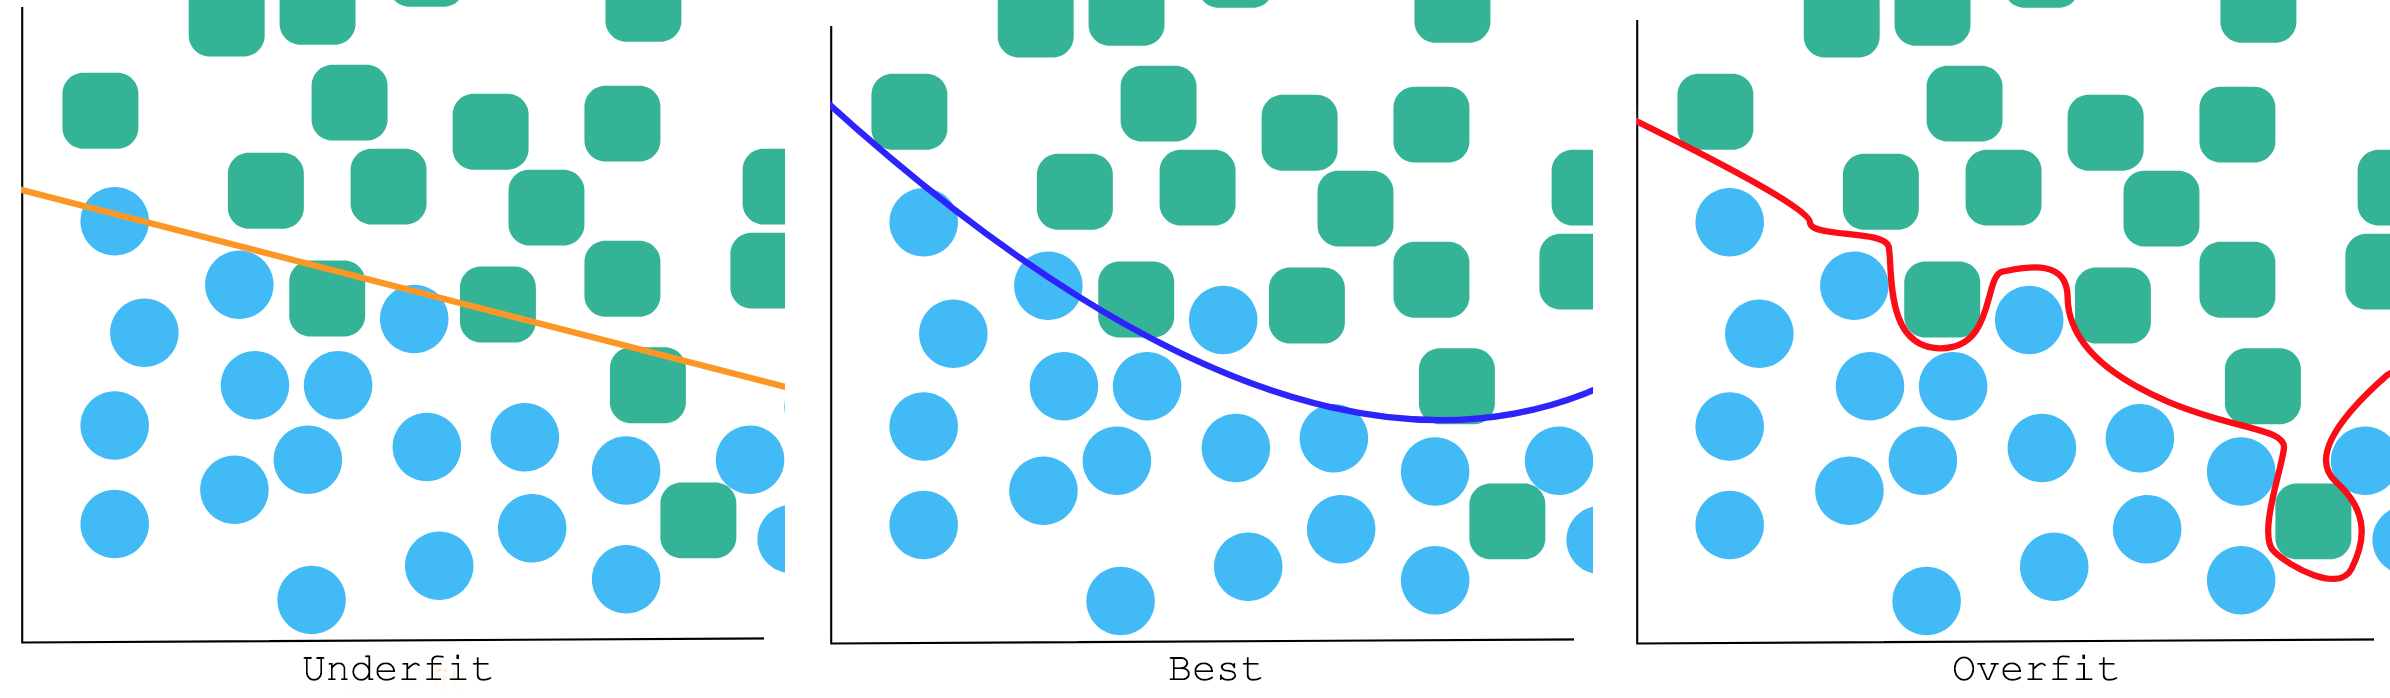
\includegraphics[width=14cm]{fitting}
		\caption{Levels of fitting for a simple classification task}
		\label{fig:fitting:1}
	\end{figure}

	\subsection{Transfer Learning}
	Transfer learning is a commonly employed technique of taking a neural network that has already been trained on a similar task, and adapting its weights to the new domain. For image classification, this is done by downloading a pre-trained model, replacing the final fully-connected softmax output layer with a new output layer and training on the new data-set. There isn't always a necessity to re-train the model, as a large portion may be general-enough to apply to the new dataset. Due to this, the fine-tuning of models varies between adapting all parameters in the network, to the last few layers, to only the final softmax layer.  \par
	The assumption that transfer learning hinges on is that the features learnt on a large data-set are general enough to transfer to a new, similar data-set. There are a number of well-known model architectures available for download, typically being trained on the \textit{ImageNet} image database. \par
	If the model is trained on a sufficiently large data-set it is true that the learnt features are usually general enough to receive good results after introducing relatively few samples from the new domain; but is not as effective as possible, especially when the new domain is significantly different from the old. As this approach requires the training of a model on a large source data-set, the user is either stuck with an existing model and no option to change, or must first train their own custom model on the large data-set first. This is a long, costly process which can be prohibitive. \par
	Despite these limitations, transfer learning is the most effective and frequently-used technique for training on a new data-set when the amount of labelled data is small, achieving better performance than training on the new labelled data alone. \par 

	\subsection{Few-Shot Learning}
	Few-shot learning is the ability to learn a new concept or idea from only a ``few'' examples. In the context of image-classification it is the ability to learn a new class from only a few example images. It's desirable to have a system that can learn from a small data-set, because -- as mentioned earlier -- it can be a long, costly process to label data-sets. \par
	The generalised description of few-shot learning for image classification is $N$-Way $K$-Shot learning, where $N$ is the number of classes between which the model is to make predictions; $K$ is the number of example images shown prior to having the model produce a prediction. Researchers tend to work on combinations of $N \in \{5, 10, 20\}$, $K \in \{1, 5\}$, regularly presented as one-shot and five-shot learning.
	
	\subsection{Meta Learning}
	Meta-learning can be described as ``learning how to learn'', and in the field of computer vision refers to having a system that is able to adapt rapidly to new classes or domains. The goal in standard machine learning is normally to have a system that can generalise between examples within a domain, leveraging information seen in the training data to gain a generalised understanding of the data distribution. Meta-learning contrasts this in that the goal is to learn from the relationship between a data distribution and learning itself -- instead of being tightly bound to one specific domain. This is a sensible objective, as it's a trick humans use to speed-up the learning of new information. After being shown a photo of the proverbial zebra, it is quicker and easier to approximately learn it as a ``stripy horse'' rather than consider it an entirely new concept. \par
	A ``meta-learner'' is a system that's responsible for this external-observation -- with the learner playing the usual role -- however there are many designs without a distinction between the two. Meta-learning for few-shot problems is generally categorised into three different approaches:
	\begin{itemize}
		\item \textbf{Optimization-based}: A model learns parameter update rules -- essentially replacing the role of an optimizer (section \ref{optimizers:1}) -- such that some good initial weights are modified rapidly and efficiently to perform well with the current set of images. These meta-learners typically employ an RNN (section \ref{rnn:1}).
		\item \textbf{Model-based}: A specific model architecture designed to handle few-shot problems by utilising some kind of memory unit -- typically an RNN (section \ref{rnn:1}), memory-network (section \ref{memory-nets:1}) or Temporal CNN\TOCITE{}.
		\item \textbf{Metric-based}: A model learns a representation of the given sample images and a method by which to compare query images with the recently-provided sample(s).
	\end{itemize}

	\subsubsection{Training}
	We will now consider the environment in which the aforementioned meta-learning approaches are trained and executed. \textit{Note that this section deals only with few-shot meta-learning for image-classification}. Having the system gain a meta-understanding of a task is almost exclusively approached in an episodic manner -- each episode consisting of conditioning a model on some examples of the task, having the model make a prediction, then updating the parameters to optimise this process. \par
	As always in image-classification tasks, the data-set $\mathcal{D}$ is split into two class-disjoint sets $\mathcal{D}_{train}$ and $\mathcal{D}_{test}$, the latter a held-out set from which the model isn't allowed to learn. Additionally, as few-shot learning requires the exposure of examples before making a prediction, each of the sets is split on an episode basis into a \textit{support} set $\mathcal{D}_{S}$ and a \textit{query} set $\mathcal{D}_{Q}$. For the case of training five-way one-shot classification, the support set will consist of one image from each of five randomly selected classes from $\mathcal{D}_{train}$, with the query set consisting of one or more images drawn from the same data-set and belonging to one of the classes found in the support set (figure \ref{fig:episode:1}). The model is shown $\mathcal{D}_S$, optimizes itself for these classes, then is shown $\mathcal{D}_Q$ for which to make a prediction. The meta-learner observes this process, and optimizes the process by which the learner adapts to each episode. \par
	Due to the episode-based training, where the system sees a ``new'' set of classes in each, the meta-learner learns class-agnostic relationships between the support-set and the query-set. This then means that the meta-learner must persist knowledge between episodes, effectively learning an episode-invariant learning technique. This is validated by presenting an episode from $\mathcal{D}_{test}$ without the meta-learner's observation. \par
	\begin{figure}[!h]
		\centering
		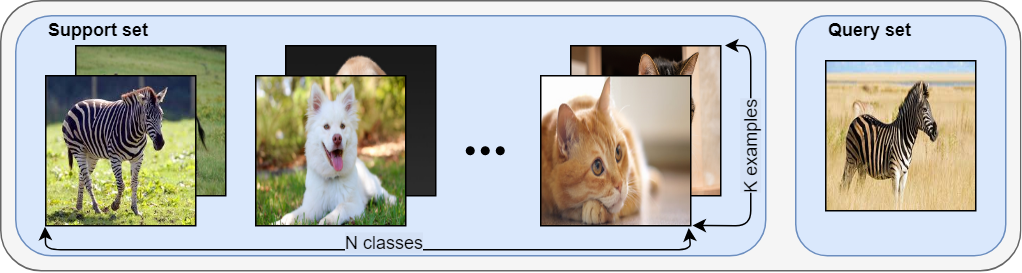
\includegraphics[width=14cm]{episode}
		\caption{An N-way K-shot training episode}
		\label{fig:episode:1}
	\end{figure}
	
	\section{Continuous Learning}
	Learning from a continuous stream of new information is a crucial milestone in the development of artificial intelligence -- especially artificial general intelligence -- as the normal offline-training procedure is impractical, and vastly different from biological neural networks. The neural networks found in the brain have the capacity for continuous learning -- the ability to learn new tasks/information without sacrificing previous skills/knowledge. ANNs don't have this capacity built-in, as the training typically occurs on a per-example (episode, image, batch, etc.) basis, with the purpose of optimising for that specific episode. It is inherent then, that a network will sacrifice its existing parameter state to perform better at the task presented. \par
	The forgetting of older knowledge when learning new information is known as \textit{catastrophic forgetting} or \textit{catastrophic interference}. It purportedly occurs when there is representational overlap inside a network between old and new information. The easiest way to gain an understanding of the new domain is to reuse that knowledge, sacrificing performance on the previous domain. This leads to an abrupt decrease in performance on the old domain, and eventually a total loss of learned knowledge. \par
	There have been many attempts at mitigating catastrophic forgetting using as number of methods (section \ref{related-cont-learning:1}) with varying degrees of success; many drawing inspiration from the brain. \par
	While this isn't a neuroscience writing (I'm certainly not qualified for that!), I will briefly mention some of the known neurophysiological functions that allow the brain to adapt quickly to new information while retaining learnt information from previous tasks. \par
	\begin{itemize}
		\item\textbf{Neurosynaptic plasticity} - The brain is particularly plastic during early development, allowing for sense-driven changes to occur on a large scale. Plasticity decreases with increasing age to provide stability, but a degree of plasticity is retained for small-scale adaptation.
		\item\textbf{Hebbian plasticity}\parencite{hebbian} - ``Neurons wire together if they fire together''\parencite{wirefire}. An observed pattern in the brain where synaptic efficacy (neuron firing strength) increases through persistent stimulation. Simply put, frequently used neural pathways gain strength and reduce plasticity.
		\item\textbf{Complementary learning systems} - As the brain's task is to both learn and memorise, it consists of two primary components relating to memory. The hippocampus rapidly encodes new memories into sparse representations for quick short-term recall with minimal interference, whereas the neocortex slowly encodes older memories into overlapping representations for long-term storage.
	\end{itemize}
	Due to the incredible capacity for the brain to deal with long-term memory without exhibiting catastrophic interference, it is reasonable that most artificial neural networks draw inspiration from biology. \par

	\section{Modern Deep Learning Architectures} \label{modern-dl:1}
	The only ANNs we've covered as of this point are \textit{fully-connected neural networks} (section \ref{fully-connected:1}) which have a very limited capacity in terms of practical use-cases, as we'll explore in this section. \par
	
	\subsection{Convolutional Neural Networks} \label{cnn:1}s
	Let us consider a fully-connected network for classification on the popular data-set MNIST (figure \ref{fig:mnist:1}), with the raw pixel values fed in one side and a class probability distribution being output. Fully-connected layers need a single column (vector) of values as inputs, so we will first ``unwrap'' the image into a long string of pixel values before feeding it in. \par
	\begin{figure}[h]
		\centering
		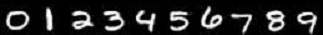
\includegraphics[width=6cm]{mnist}
		\caption{Ten examples from the MNIST dataset}
		\label{fig:mnist:1}
	\end{figure}
	Each input pixel would then be mapped by a distinct neuron weight in the first layer, which is problematic. Following the "importance weighting" interpretation introduced in section \ref{fully-connected:1}, the network must consider each input pixel individually with regards to its importance in the classification prediction. The same input image shifted by one pixel in any direction will likely produce very different results. This problem is inherent to fully-connected layers, and is best addressed by \textit{convolutional layers}. \par
	We would instead prefer to see the image in a more global context, where we can learn about the presence or absence of features throughout the image. It's easier to describe the number eight as ``one circular thing on top of another circular thing'' than by raw pixel intensities. This was the work of hand-engineered \textit{kernels} for a long time prior to the resurgence of neural networks -- see figure \ref{fig:hand-eng-kernels:1} for examples of hand-engineered kernels and their effects. As kernels are a fundamental concept for convolutional neural networks, we'll now go into some detail. \par
	\begin{figure}[!h]
		\centering
		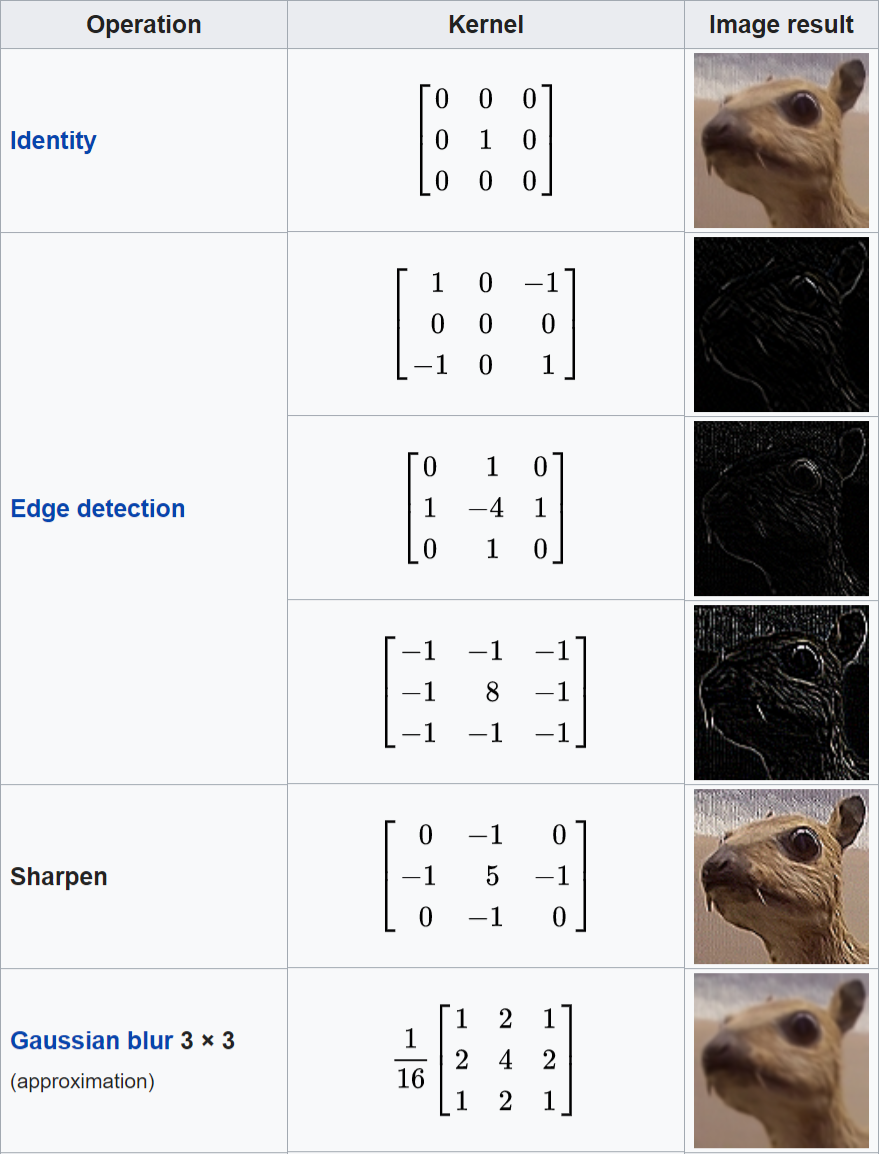
\includegraphics[width=8cm]{handengkernels}
		\caption{Hand-engineered image kernels}
		\label{fig:hand-eng-kernels:1}
		\textit{Source: https://en.wikipedia.org/wiki/Kernel\_(image\_processing)}
	\end{figure}
	A kernel -- also known as a filter -- is a (typically square) matrix that is convolved over an input image to produce another image which contains some locally-aggregated information. It can be thought of as a window that slides over the image, seeing it in small sections. At each position the values in the input are multiplied by the corresponding point in the kernel, and the output value is their sum. Figure \TOCITE{} shows a 2x2 kernel applied to a the pixel values of a very small input image, and the resultant values. Their applicability to neural networks is very convenient, as all we need to do is replace the hand-engineered values with learnt weights and we have the makings of a convolutional layer. As discussed in section \ref{hand-eng:1}, hand-engineered features are usually of limited capacity, with data-driven features being more powerful. \par
	The outputs of a single kernel 3x3 convolutional layer are an image-like matrix which contains locally-aggregated information from the input image. As the kernel is 3x3 pixels, the \textit{effective receptive field} size at this point is 3x3 pixels. That is, the features in the outputs correspond to a region of three pixels in each direction. If the outputs of this layer are fed into another layer of the same size, the effective receptive field size at this extra layer will be 5x5 pixels. The trend of an increasing receptive field continues for more layers, which has great consequences -- the further into a network of convolutional layers, the more global the information as the deeper filters can see more of the input image features. \par
	It's important now to discuss what ``features'' are, as they're a key concept that have a fuzzy meaning. Image features extracted by data-driven convolutional kernels are unintuitive by nature, but we can build a sufficient understanding logically. Consider that through training our network, filters will be developed that respond to important features. These features will likely be things like horizontal lines; vertical lines; and soft gradients -- simple features. Subsequent layers will be dealing with not images but extracted features, so they will be responding to \textit{combinations} of features -- things like corners and more complex edges. As we proceed further into the network, the features learnt get more complex until we have filters responding to things like dog noses, text, wheels, etc. \par
	With this knowledge that the depth of a neural network corresponds to its global understanding and its ability to learn complex features, it makes sense that modern convolutional neural networks are quite deep -- sometimes into the hundreds. For the task of image classification, the missing link in the chain is how we produce the probability over the classes -- take the outputs of the final convolutional layer, ``unwrap'' it as we did for the input image, and pass it through a fully-connected layer to produce the right number of output values. \par
	
	\subsection{Recurrent Neural Networks}\label{rnn:1}
	\TODO{Week 4}
	Nothing covered so far has had the capacity to work on temporal data; Recurrent Neural Networks (RNNs) address this. We have only seen two sets of values relating to a neural network -- weights, which are the network's ``intelligence''; and activations, which are the neurons' responses to the given inputs. Only the weights persist between runs, but don't have the capacity to retain information about individual samples (if they do, they've overfit!). \par
	For a neural network with a single hidden-layer, the activations at time $t$ are $h = \sigma(\bm{W}\bm{x}_t)$ for some input $\bm{x}_t$, weights $\bm{W}$, and activation function $\sigma$. RNNs work by recursively passing their hidden state through time-steps, weighted by learnt values. This can be expressed mathematically as 
	\begin{align}
		\bm{h}_{t} = \sigma(\bm{W}\bm{x}_t + \bm{U}\bm{h}_{t-1})
	\end{align}
	where $\bm{U}$ is a learnt matrix which filters and scales the hidden state values passed between time-steps. The recurrent design of this relationship means that not only will time-step $t$ contain information from time-step $t-1$, but $t-2, t-3, ...$ Figure \TOCITE{} shows a very simple RNN. Note that we haven't discussed how to trigger an RNN to stop -- this is purposefully omitted as it's outside the scope of this writing. \par
	By their design, RNNs are able to consider all prior information when making a prediction. This makes them a perfect candidate for time-series or arbitrary length sequence data such as text, weather predictions, speech-recognition etc.
	
	\subsubsection{Exploding/Vanishing Gradients}
	When training an RNN, you typically need to see the entirety (or at least a large portion) of its outputs to compute the loss -- e.g. we can't assess how well it constructed a sentence until we can see the whole sentence. The training error is back-propagated through time from the last of the output sequence to the first of the input sequence (see the red arrows in figure \TOCITE{}). \par
	As the gradients must be passed a long way, it is easy to imagine that we may end up with compounding errors, resulting in numerical instability. Gradients are particularly susceptible to this -- with the relationship between layers being multiplicative, any consecutive operations on values less than 1 approach zero, and any consecutive operations on values greater than 1 approach $\infty$. These problems are known respectively as the vanishing gradient problem, and the exploding gradient problem. Figure \ref{fig:multi-sigmoids:1} demonstrates this problem: with the sigmoid function being applied repeatedly we see that the output values ``flatline'' with the gradient rapidly approaching zero. As the gradients are used to propagate training error, no gradient means no learning.
	\begin{figure}[h]
		\centering
		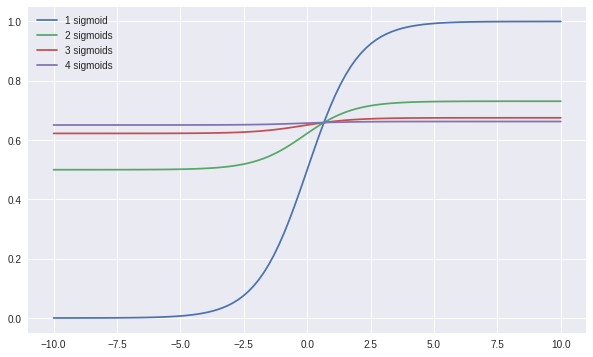
\includegraphics[width=10cm]{multi-sigmoids}
		\caption{The effects of applying the sigmoid function repeatedly}
		\label{fig:multi-sigmoids:1}
	\end{figure}
	\subsubsection{Long Short-Term Memory Units}
	Long Short-Term Memory Units (LSTMs) were proposed as a solution to the aforementioned gradient problems inherent to RNNs. They have become so prolific and successful that usage of the acronym RNN generally refers to an LSTM instead. LSTMs mitigate the exploding/vanishing gradients problem by containing information outside of the normal hidden state of the network; the RNN approach doesn't really allow for dynamic usage of the hidden state. \par
	LSTMS introduce a memory structure referred to as a \textit{gated cell}, which is similar to Random Access Memory on a typical computer -- information can freely be written, read, and erased out of order. However, while RAM supports digital reading/writing/erasing, LSTMs allow for \emph{analog} memory access -- data is changed and read to varying degrees in a differentiable process. There are a handful of variants on the LSTM which are growing in popularity, but as the internal workings of those, and LSTMs are too complex to discuss in this writing, swe won't explore them any further. \par
	
	\subsection{Memory Networks}\label{memory-nets:1}
	As regular feed-forward don't have any memory units but RNNs do, they have been used for tasks where memory is required, but not for necessarily sequential data. Memory networks address this by augmenting regular neural networks to have an addressable external memory unit. They operate in a very similar manner to LSTMs, in that they have the equivalent to gates managing the read/write/erasure of elements in the memory unit. We will briefly touch on how a memory network functions as it has great relevance to few-shot learning, where memory of past examples is helpful, but doesn't have a strict temporal relationship. \par
	A high-level view of memory networks (as shown in figure \TOCITE{}) is as follows:
	\begin{itemize}
		\item \textbf{Memory} - An indexed array of vectors representing the currently-stored information.
		\item \textbf{Input map} - Transforms inputs to a unified internal feature representation.
		\item \textbf{Generalisation component} - Updates old memories given new input. Referred to as ``generalisation'' as this is responsible for compressing and generalising old memories into new representations.
		\item \textbf{Output map} - Produces an output given the new input and the state of memory.
		\item \textbf{Response component} - Converts the output into the external representation, such as text, prediction probability distribution, etc. 		
	\end{itemize}
	Memory networks have had significant success, and offer a practical alternative to RNNs when working with any variable-length data -- time-series based or not.
	
	\chapter{Related Works} \label{related:1}
	\TODO{Week 5}
	Approaches in meta learning with neural networks are generally grouped into three categories.
	\subsection{Model Based} \label{related-meta-modl:1}
	\TODO{Week 5}
	
	\subsection{Metric Based} \label{related-meta-metr:1}
	\TODO{Week 6}
	\subsection{Optimization Based} \label{related-meta-opt:1}
	\TODO{Week 7}
	\section{Continuous Learning} \label{related-cont-learning:1}
	\TODO{Week 8}
	\chapter{Proposal}
	\TODO{Week 9}
	\TODO{Week 10}

	\printbibliography
	
	


\end{document}
